\section{Experiments}

\subsection{Comparison metrics}

Biometric systems have transformed the landscape of identity verification and access control, offering a reliable and efficient way to authenticate individuals based on their unique physical or behavioral traits \cite{jain2007handbook}. These systems leverage characteristics like fingerprints, iris patterns, voiceprints, facial features, or gait patterns to establish an individual's identity \cite{bolle2013guide}. However, even with their advancements, biometric systems are not immune to errors and uncertainties. Therefore, it becomes essential to evaluate their performance using well-defined metrics.

The evaluation of biometric systems involves analyzing various aspects of their performance, including accuracy, reliability, and security. Among the key metrics used for this purpose are the False Acceptance Rate (FAR), False Rejection Rate (FRR), and Equal Error Rate (EER)\cite{benchmarks}. These metrics provide valuable insights into the system's ability to correctly identify and authenticate individuals while managing the delicate balance between accepting impostors (false acceptance) and rejecting legitimate users (false rejection).

The False Acceptance Rate (FAR) signifies the probability of the system mistakenly accepting an impostor or granting access to an unauthorized individual and can be described by the equation \ref{eq:far}. Conversely, the False Rejection Rate (FRR) reflects the likelihood of the system erroneously rejecting a legitimate user or denying access to an authorized individual and can be expressed by the equation \ref{eq:frr}. Both FAR and FRR play crucial roles in assessing system performance, as they directly impact the security and usability of biometric systems.

The Equal Error Rate (EER) is another vital metric that offers a balanced evaluation of system performance. It represents the threshold at which the FAR and FRR intersect, indicating the point where the rates of false acceptance and false rejection are equal. EER serves as a benchmark for comparing different biometric systems, enabling system administrators to select an optimal threshold that balances security and usability considerations\cite{benchmarks}.

A comprehensive understanding of FAR, FRR, and EER is essential in evaluating the performance of biometric systems. By quantifying the rates of false acceptance and false rejection, these metrics facilitate the identification of vulnerabilities, system limitations, and areas for improvement. Additionally, they contribute to the establishment of standards, benchmarks, and best practices for deploying reliable and efficient biometric authentication systems.

By gaining insights into these metrics, researchers, practitioners, and decision-makers can make informed choices regarding the design, implementation, and enhancement of biometric systems. Additionally, a deeper understanding of FAR, FRR, and EER empowers stakeholders to evaluate the effectiveness, reliability, and security of biometric technologies in real-world applications.

Other studies have already used these metrics to evaluate the performance of biometric systems. For example, \cite{deep_learning} used FAR, FRR, and EER to compare the performance of similar techniques for adressing the improvement of their new deep learning-based approach for keystroke dynamics authentication. Similarly, \cite{typing_patterns} used FAR and FRR to evaluate the performance of some of the work done in the field of keystroke dynamics authentication as can be seen in Figure \ref{fig:far_frr}.

\begin{figure}
    \centering
    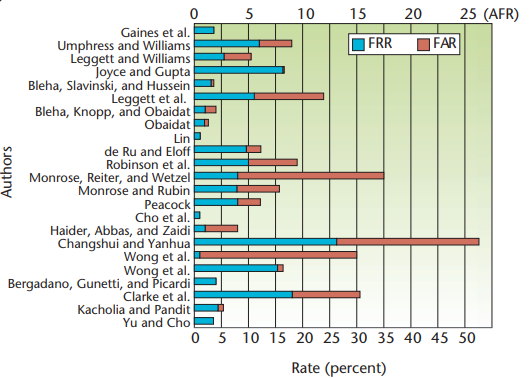
\includegraphics[width=0.5\textwidth]{images/studies.png}
    \caption{FAR and FRR for different approaches to keystroke dynamics authentication \cite{typing_patterns}}
    \label{fig:far_frr}
\end{figure}